\chapter{Problem description and Related work}
\label{sec:problem_description}
\section{Problem description}

Standard reinforcement learning approaches aim to find policies which maximize the expected cumulative reward.
However, this approach neither takes into account variability of the reward around its mean
neither sensitivity of the policy to modelling errors.\\
In this thesis, we change the objective function of the
standard RL approach to one that optimizes another metric of the reward distribution which
takes into account the risk of the actions taken by the agent.
While several metrics have been designed to assess risk, we will focus on a particular risk metric
called Conditional Vale at Risk (CVaR).\\
We, thereby, present a RL algorithm that aims to find policies with optimal CVaR.

\subsection{Reinforcement Learning}

Reinforcement learning is an approach to learn a mapping from situations or states to actions so as to maximize 
a numerical reward signal. The learner or \textit{agent} is not told which actions to take
but instead must discover which actions yield the most reward by trying them. In most of the cases,
actions may affect not only the immediate reward but also the next state and consequently, all subsequent rewards.
These two characteristics—trial-and-error search and delayed reward—are the two most important
distinguishing features of reinforcement learning \citep{Sutton1998}.

\subsubsection{Markovian Decision Processes (MDPs)}
We formalize the problem of RL by using the framework of Markov decision processes (MDPs)
to define the interaction between a learning agent and its environment in terms of states,
actions and rewards.

MDPs  are discrete-time stochastic control processes which provide a
mathematical framework for modeling sequential decision making in situations where outcomes are
partly random and partly under the control of a decision maker and where actions influence not only immediate rewards,
but also future ones.\\
An MDP is defined by a tuple ($\mathcal{S,A},R,P,\gamma$), where $\mathcal{S,A}$ are the
state and action spaces respectively, $R(x,a)$ is the reward distribution, $P(\cdot |x,a)$ is
the transition probability distribution and $\gamma \in [0,1]$ is the discount factor. 

State transitions of an MDP satisfy the Markov property, in which
the set of transition probabilities to next states depend only on the current state and action of the system,
but are conditionally independent of all previous states and actions. Hence, the state must
provide information about all aspects of the past agent-environment interaction that
make a difference for the future.

Solving an MDP involves determining a sequence of policies $\pi$ (mapping states to actions)
that maximize an objective function.
A commonly considered class of policies in literature are the class of Markovian policies $\Pi_M$ where
at each time-step \textit{t} the policy $\pi_t$ is a function that maps state $x_t$ to 
the probability distribution over the action space $\mathcal{A}$. 
In the special case when the policies are time-homogeneous, i.e. $\pi_j = \pi \; \forall j \geq 0$ then the
class of policies is known as stationary Markovian $\Pi_{M,S}$.\\
This set of policies, under which actions only depend on current state information and
its state-action mapping is time-independent, makes the problem of solving for an optimal policy more
tractable and common solution techniques involve dynamic programming algorithms \citep{Bertsekas1995}
such as Bellman iteration.\\
When the objective function is given by a risk-neutral expectation of cumulative reward,
i.e.:
\begin{equation}
    \underset{\pi \in \Pi_H}{\min} \mathbb E  \big [  \sum_{t=0}^{\infty} \gamma^t R(x_t,a_t) | x_0, a_t \sim \pi_t(\cdot |h_t)  \big]
\end{equation} 

where $ \Pi_H$ represents the set of all history-dependant policies,
the Bellman's principle of optimality \citep{Bertsekas1995} shows that the optimal
policy lies in the class of stationary Markovian policies $\Pi_{M,S}$

When dealing with other types of objective functions that aim towards more risk-sensitive
policies, these nice properties doesn't normally hold
and require extra mathematical formulations, such as MDP state augmentation \citep{Chow2015}.



\section{Risk}
Standard reinforcement learning agents aim to maximize the expected cumulative reward and hence
do not take risk into account. In some scenarios the shape of the reward distribution might be unimportant,
since highly different distributions still can have same expectation. However, in real world scenarios, 
in  when catastrophic losses can occur, risk must be taken into account.\\
We can find 3 types of strategies with respect to risk, namely \textit{risk neutral, risk averse} and \textit{risk seeking}

As an example, suppose a participant in a game is told to choose between two doors.
One door hides 1000CHF and the other 0CHF. The host also allows the contestant to 
take 500CHF instead of choosing a door. The two options (choosing between door 1 and door 2, or taking 500CHF)
have the same expected value of 500CHF. But it can clearly be seen that the risk among two options is different.
Since the expected value is the same, risk neutral contestant is indifferent between these choices.
A risk-seeking contestant will maximize its utility from the uncertainty and hence choose a door,
whereas the risk-averse contestant  will accept the guaranteed 500CHF.


In this thesis we present an algorithm to find risk-sensitive policies
that maximize the CVaR of the reward distribution.

\subsection{Conditional Value-at-Risk (CVaR)}

Let Z be a bounded-mean random variable, i.e $\mathbb E[|Z|] < \infty$, on a probability space 
$(\Omega, \mathcal{F}, \mathbb P)$, with cumulative distribution
function $F_Z(z) = \mathbb P (Z \leq z)$. We interpret Z as the reward distribution and for convenience 
we assume that is a continuous random variable meaning that $F_Z(z)$ is everywhere continuous.
The value-at-risk (VaR) at confidence level $\alpha \in (0,1) $ is the $\alpha$-quantile of Z, i.e.:

\begin{equation}
    \text{VaR}_\alpha (Z) = F_Z^{-1}(\alpha)= \inf \{ z \hspace{1mm} | \hspace{1mm}F_Z(z) \geq  \alpha  \}
\end{equation}

The conditional value-at-risk (CVaR) at confidence level $\alpha \in (0,1) $ is defined as
the expected reward of outcomes worse than the $\alpha$-quantile ($\text{VaR}_\alpha$):
\begin{equation}
    \text{CVaR}_\alpha (Z) = \mathbb E [Z | Z \leq \text{VaR}_\alpha]= \frac{1}{\alpha} \int_{0}^{\alpha} F^{-1}_Z(\tau) d\tau=\frac{1}{\alpha} \int_{0}^{\alpha} \text{VaR}_\tau (Z) d\tau \label[]{eq:cvar_defs}
 \end{equation}
The last equality, known as the Acerbi's integral formula for CVaR (Proposition 3.2 in \citet{Acerbi2002}),
interprets $\text{CVaR}_\alpha$ as the integral of all the quantiles below
the corresponding quantile level $\alpha$ and will become useful later.   \\
While both VaR and CVaR are risk measures, CVaR has superior mathematical properties 
(monotonicity, translation invariance, positive homogeneity and subadditivity; see \citet{Artzner1999})
which makes CVaR computation and optimization far easier compared to VaR \citep{Rockafellar2000}.
In addition, CVaR takes into account the possibility of tail events where losses exceeds VaR whereas VaR
is incapable of distinguishing situations beyond it.

\citet{Rockafellar2000} also showed that CVaR is equivalent to the solution of
the following optimization problem:

\begin{equation}
    \text{CVaR}_\alpha (Z) = \underset{\nu} \max \big\{\nu + \frac{1}{\alpha} \mathbb E_Z[[Z- \nu]^-]\big\} \label{eq:rockafellar}
\end{equation}

where $(x)^- = \min(x,0)$.\\
In the optimal point it holds that $\nu^*=\text{VaR}_\alpha(Z)$.

A useful property of CVaR, is its alternative dual representation \cite{Artzner1999}:
\begin{equation}
    \text{CVaR}_\alpha (Z) = \underset{\xi \in U_{\text{CVaR}} (\alpha, \mathbb{P})} \min \mathbb E_\xi[Z] \label{eq:dual_cvar}
\end{equation}

where $\mathbb E_\xi[Z]$ denotes the $\xi$-weighted expectation of $Z$, and the risk envelope $U_\text{CVaR}$ is
given by:
\begin{equation}
    U_{\text{CVaR}}(\alpha, \mathbb{P}) = \Big\{\xi | \xi(w)  \in \big [ 0, \frac{1}{\alpha} \big ], \int_{w\in\Omega} \xi(w)\mathbb{P}(w)dw=1   \big ] \Big\}
\end{equation}

Thus, the CVaR of a random variable may be interpreted as the worst case expectation of $Z$, under
a perturbed distribution $\xi \mathbb{P}$.

Our goal in this thesis is to find policies that maximize the CVaR of the 
return distribution i.e.:
\begin{equation}
    \arg \underset{\pi}\max \text{CVaR}_\alpha [Z (x, \pi(x))] \quad \forall x \in \mathcal{X}
\end{equation}

To this end, we present an algorithm for CVaR optimization using a \textit{distributional} variant 
of the deterministic policy gradient algorithm.
The word \textit{distributional} emphasizes that our approach takes inspiration from the
recent advances in distributional RL 
\citep{Bellemare2017,Dabney2018a,Dabney2018b} to estimate the full
\textit{value distribution} (i.e. the distribution of the random return received by a RL agent).
Having an estimation of the true value distribution, we compute the CVaR of the current policy
via sampling from the estimated value distribution and we move the current policy
towards maximizing it via stochastic gradient ascent.\\
\todo{should I repeat all this? Specify that they are NN's actor/critic?}
The CVaR dual formulation and the Acerbi's integral formula \ref{eq:cvar_defs} presented above,
will be useful to derive our approach to compute the CVaR 
from parameterized inverse cumulative distributions.

\begin{figure}[ht]
    \centering
    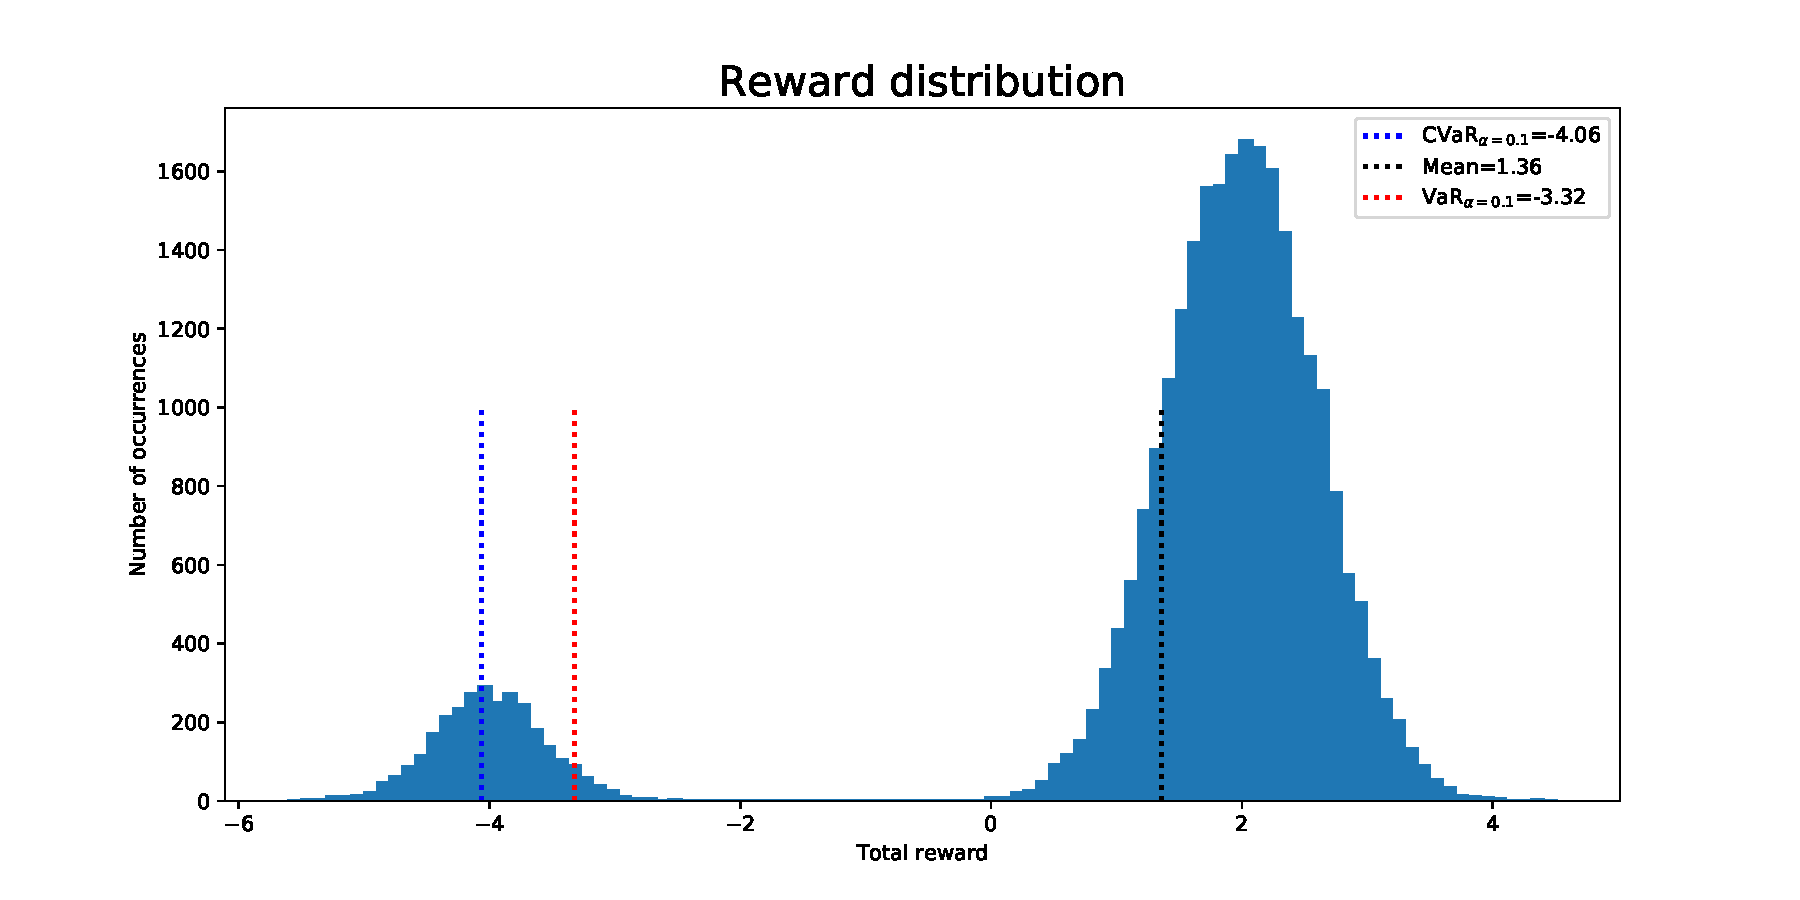
\includegraphics[width=0.8\textwidth]{images/cvar_motivation2.pdf}
    \caption{Histogram showing VaR,mean and CVaR of a sampled probability distribution.
    The image shows that the mean doesn't take into account low probability events and 
    the flow of
    the VaR as a risk metric, since we could move the left-most mode to minus infinity
    and the VaR will remain the same, whereas the CVaR would change with the shift. }
    \label{cvar_cheetah}

\end{figure}

